

\subsection{Experiment Settings}

\subsubsection{Environment}
We benchmark the implementation in two execution environments: the
cycle-accurate \texttt{hexagon-sim} shipped with the Qualcomm Hexagon SDK, and
the on-device cDSP path accessed from an Android host through FastRPC. The
simulator binary is executed through the H2 minimal hypervisor and its booter
entrypoint. The cDSP image is compiled with the same \texttt{hexagon-clang}
configuration as the simulator binary, while the Android host benchmark is
cross-compiled with the NDK Bionic toolchain.

% The decoder under test is organized into three sibling C source trees that
% export the same \texttt{code\_decode} interface: a portable scalar baseline, an
% HVX-assisted path used as the NPU-supported variant in Tables~3--6, and a
% non-constant-time worker-best path used for the on-device throughput results in
% Table~7. These trees are shared by the simulator, host benchmark, and FastRPC
% cDSP builds, ensuring that each reported number is obtained from the same
% bit-identical decoder source for the corresponding backend.

\subsubsection{ FastRPC communication with the NPU}
In the execution context, the CPU requires a communication protocol to offload specific tasks to the NPU. Since the CPU and NPU operate in different execution domains, the CPU cannot directly invoke NPU kernels as ordinary local functions. Instead, it relies on a runtime communication mechanism, namely FastRPC~\cite{Qua18HexagonDSP}, to transfer control information, pass buffer descriptors, and synchronize task execution.

In this workflow, the CPU first prepares the input data in a shared I/O buffer that is accessible by both the CPU and the NPU. Rather than copying large data through the control path, the CPU passes only lightweight metadata, such as buffer handles, data sizes, and task parameters. The FastRPC stub on the CPU side marshals these arguments and forwards the request to the NPU-side runtime. The NPU runtime then dispatches the corresponding kernel, reads the input from the shared buffer, performs the computation, and writes the result back to the output buffer. Finally, the completion status is returned to the CPU, which synchronizes and reads the output. The complete workfow is visualized in figure~\ref{fig:fastrpc_base_NPU}

Unfortunately, each initialization incurs a non-negligible overhead, averaging
around $500~\mu$s, which makes per-decode initialization undesirable. To address
this issue, we batch multiple decoding instances and offload them to the NPU in
a single communication round, thereby amortizing the extra cost. This strategy
is natural in practical applications, where devices often process continuously
arriving data, especially in streaming video workloads. The detailed measurement is given in~\ref{}



\begin{figure}[h]

\centering
\begin{tikzpicture}[
  cpuNode/.style={
    draw=blue!70!black, fill=blue!8, text=blue!60!black,
    rounded corners=6pt, minimum width=3.8cm, minimum height=1.1cm,
    align=center, font=\small\bfseries, line width=0.6pt
  },
  bufNode/.style={
    draw=cyan!70!black, fill=cyan!8, text=cyan!60!black,
    rounded corners=6pt, minimum width=3.8cm, minimum height=1.3cm,
    align=center, font=\small\bfseries, line width=0.6pt
  },
  stubNode/.style={
    draw=magenta!70!black, fill=magenta!8, text=magenta!60!black,
    rounded corners=6pt, minimum width=3.8cm, minimum height=1.3cm,
    align=center, font=\small\bfseries, line width=0.6pt
  },
  drvNode/.style={
    draw=yellow!50!black, fill=yellow!12, text=yellow!40!black,
    rounded corners=6pt, minimum width=3.8cm, minimum height=1.1cm,
    align=center, font=\small\bfseries, line width=0.6pt
  },
  dspNode/.style={
    draw=red!70!black, fill=red!8, text=red!60!black,
    rounded corners=6pt, minimum width=3.8cm, minimum height=1.1cm,
    align=center, font=\small\bfseries, line width=0.6pt
  },
  kernNode/.style={
    draw=green!60!black, fill=green!8, text=green!45!black,
    rounded corners=6pt, minimum width=3.8cm, minimum height=1.1cm,
    align=center, font=\small\bfseries, line width=0.6pt
  },
  solidArr/.style={-{Stealth[length=5pt,width=4pt]}, thick},
  dashArr/.style={-{Stealth[length=5pt,width=4pt]}, thick, dashed, gray!70},
  lbl/.style={font=\scriptsize, fill=white, inner sep=2pt}
]

% ── Top-side nodes ────────────────────────────────────
\node[cpuNode]  (cpu)  at (0,    0  ) {CPU Application};

\node[bufNode]  (buf)  at (0,   -2.4)
  {Shared I/O Buffer\\
   {\footnotesize\mdseries\color{cyan!60!black}DMA-accessible, zero-copy}};

\node[stubNode] (stub) at (0,   -5.0)
  {FastRPC Stub\\
   {\footnotesize\mdseries\color{magenta!60!black}User-space proxy, marshals args}};

% ── Draw subsystem background BEFORE bottom nodes ─────
\draw[
  draw=gray!60,
  dashed,
  rounded corners=8pt,
  fill=gray!10
] (-6.75,-8.95) rectangle (6.75,-6.95);

\node[
  font=\scriptsize\itshape,
  text=gray!70
] at (-5.35,-7.15) {NPU subsystem};

% ── Bottom-side nodes ─────────────────────────────────
\node[drvNode]  (drv)  at (-4.4, -8.0)
  {FastRPC Driver\\
   {\footnotesize\mdseries\color{yellow!40!black}Kernel driver, IPC}};

\node[dspNode]  (dsp)  at ( 0,   -8.0)
  {NPU Runtime\\
   {\footnotesize\mdseries\color{red!60!black}Schedules compute tasks}};

\node[kernNode] (kern) at ( 4.4, -8.0)
  {Kernel Execution\\
   {\footnotesize\mdseries\color{green!45!black}Runs NN / signal kernels}};

% ── Forward execution path ────────────────────────────
\draw[solidArr, blue!70!black]
  (cpu.south) -- (buf.north)
  node[lbl, midway, right=5pt] {write input};

\draw[solidArr, cyan!70!black]
  (buf.south) -- (stub.north)
  node[lbl, midway, right=5pt] {invoke with buffer};

\draw[solidArr, magenta!70!black]
  (stub.south) -- ++(0,-0.6) -| (drv.north);

\draw[solidArr, yellow!50!black]
  (drv.east) -- (dsp.west);

\draw[solidArr, red!70!black]
  (dsp.east) -- (kern.west);

% ── Buffer handle / descriptor path ───────────────────
\coordinate (A) at (buf.east);
\coordinate (B) at (6.9, -2.4);
\coordinate (C) at (6.9, -8.0);
\coordinate (D) at (kern.east);

\draw[dashArr]
  (A) -- (B) -- (C) -- (D);

\node[lbl, rotate=90] at ($(B)!0.5!(C)$)
  {buffer handle / descriptor};

% ── Completion / status return path ───────────────────
\coordinate (E) at (kern.south);
\coordinate (F) at (4.4,  -9.4);
\coordinate (G) at (-7.0, -9.4);
\coordinate (H) at (-7.0, -5.0);
\coordinate (I) at (stub.west);

\draw[dashArr]
  (E) -- (F) -- (G) -- (H) -- (I);

\node[lbl] at ($(F)!0.5!(G)+(0,-0.05)$) [below=2pt]
  {completion / status};

\end{tikzpicture}
\label{fig:fastrpc_base_NPU}
\caption{FastRPC-based NPU task execution flow.}
\end{figure}

% \subsubsection{Data generation.}
% Decoding correctness is anchored on a small, deterministic fixture corpus rather
% than on a live encoder. For each parameter set, a host generator
% \texttt{gen\_hqc\{1,3,5\}\_decode\_fixture.c} is built with system
% \texttt{gcc}, linked against the portable scalar \texttt{code\_encode} /
% \texttt{code\_decode} chain, and executed once on the host to emit a C file that
% is then checked into the repository and compiled into every benchmark binary.

% The generator follows three steps for each of the $N_{\mathrm{fix}}=16$
% entries in the corpus. First, a 32-bit \texttt{xorshift32} pseudo-random
% generator, seeded with the fixed value \texttt{0x128c0de5}, fills the message
% buffer of length \texttt{PARAM\_K} bytes. Second, the message is passed through
% \texttt{code\_encode} to obtain a clean concatenated codeword of length
% \texttt{VEC\_N1N2\_SIZE\_BYTES}. The fixture at index $f$ then has exactly
% $f \bmod (\delta+1)$ Reed--Solomon symbol errors injected into the codeword,
% with both the symbol positions and the per-symbol error patterns drawn from the
% same PRNG stream. The corpus therefore sweeps the full $0,\ldots,\delta$
% error-count regime, including the boundary case $f=\delta$ at which the
% Reed--Solomon decoder operates at its design limit. Third, the generator
% immediately calls \texttt{code\_decode} on the corrupted codeword and aborts
% unless the recovered message matches the original message byte-for-byte. This
% roundtrip is a precondition for emitting the fixture file.

% \paragraph{Correctness oracle.}
% Each generated fixture file exposes four constant arrays:
% \begin{itemize}
%     \item \texttt{hqc\{N\}\_fixture\_messages[16][PARAM\_K]}: the original
%     plaintexts;
%     \item \texttt{hqc\{N\}\_fixture\_codewords[16][VEC\_N1N2\_SIZE\_BYTES]}:
%     the post-error codewords actually fed to the decoder under test;
%     \item \texttt{hqc\{N\}\_fixture\_expected\_messages[16][PARAM\_K]}: the
%     recovered plaintexts produced by the scalar reference decoder at generation
%     time;
%     \item \texttt{hqc\{N\}\_fixture\_rs\_symbol\_errors[16]}: the number of
%     Reed--Solomon symbol errors injected into each entry.
% \end{itemize}

% Because the corpus is deterministic, checked in, and compiled into every
% binary, the cycle counts in Tables~3 and~4, the latency and energy numbers in
% Table~5, and the CPU utilization in Table~6 are reproducible bit-for-bit across
% machines and across the simulator, host, and FastRPC paths. Each benchmark
% binary additionally calls \texttt{memcmp} between the decoded output and the
% entry's \texttt{expected\_messages} after every decode and prints an explicit
% \texttt{result=PASS} or \texttt{result=FAIL} on its final line; a
% \texttt{FAIL} result invalidates the run and is treated as a hard failure rather
% than repqqqlorted as a measurement1g.

\subsubsection{Measurement metrics}
We report four complementary metrics to evaluate the proposed implementation:
simulated processor cycles, real-device latency, device energy, and CPU
utilization.

\paragraph{Hexagon Pcycles.}
To avoid simulator startup and teardown effects, we use a paired measurement
strategy. We measure both a one-iteration and a three-iteration run, subtract the
former from the latter, and normalize by the number of additional decodes:
\[
    \mathrm{Pcycles/decode}
    =
    \frac{
        \mathrm{Pcycles}_{T=3}
        -
        \mathrm{Pcycles}_{T=1}
    }{
        (3-1) \times N_{\mathrm{fix}}
    } .
\]
The same estimator is used for both the scalar baseline and the NPU-supported
variant, as well as for the substage breakdown.

\paragraph{Real-device latency and energy.}
On the Android device, we measure wall-clock latency around the decoding loop
and divide by the total number of decodes. Energy is measured by sampling device
power-supply voltage and current during execution, integrating power over time,
and normalizing by the number of decodes. We disable \texttt{qprof} during
energy measurement to avoid perturbing power and clock behavior.

\paragraph{CPU utilization.}
We measure the CPU cost paid by the Android host process under each backend. In
the CPU-scalar configuration, this is the process that runs the scalar decoder
directly on the Kryo CPU. In the NPU-supported configuration, it is the same
host-side benchmark process acting as a FastRPC dispatcher: it submits batched
decode work to the cDSP and waits for completion. The measurement wrapper
samples \texttt{/proc/<pid>/task/*/stat} while the process is alive, sums the
user and system jiffies across all of the process threads, and converts the
tick delta using \texttt{getconf CLK\_TCK}. We then normalize the resulting host
CPU time in two ways. The process CPU percentage divides host CPU time by the
wall-clock interval, so \(100\%\) corresponds to one fully loaded CPU core on
the Snapdragon 8 Gen 2 platform rather than to the entire multi-core SoC. The
CPU ms/decode metric divides the same host CPU time by the number of completed
decodes. Finally, CPU reduction compares CPU ms/decode against the CPU-scalar
baseline and therefore quantifies host-side offload only; NPU-supported decoding
still consumes Hexagon cycles on the cDSP, which are reflected separately in the
latency and energy measurements.
% \paragraph{FastRPC boundary overhead.}
% FastRPC boundary overhead in Table~\ref{tab:fastrpc-boundary-overhead} is isolated with three microbenchmarks built
% from the same FastRPC stub as the throughput runs. The Ping $\mu$s/RPC column
% uses a no-op remote call to measure the per-call boundary cost in isolation. The
% Decode-one $\mu$s/decode column measures the worst case in which exactly one
% decode is dispatched per remote call. The Batched $\mu$s/decode column reuses
% the worker-best codeword count from Section~\ref{} and reports the amortized
% per-decode cost. The Decode-one slowdown column is the ratio between the second
% and third measurements and quantifies how much the worker-best batching
% amortizes the FastRPC boundary.


\subsection{Simulation Results}

The simulator benchmark is conducted on the current 256-fixture decoding corpus
for each HQC parameter set and reports Hexagon processor cycles (Pcycles).
Instead of reporting raw \texttt{hexagon-sim} totals as the main result, we use
the paired \(T=1\) and \(T=3\) runs to expose the actual normalized cost. The
\(\Delta\) columns in Table~\ref{tab:sim-pcycles-full} are the difference between
the three-iteration and one-iteration runs; the estimated cycles per decode are
then obtained by dividing \(\Delta\)Pcycles by \(\Delta\)decodes. This presentation
keeps the fixed simulator/setup overhead separate from the per-decode estimate.

\begin{table}[htbp]
\centering
\renewcommand{\arraystretch}{1.15}
\small
\begin{tabular}{|l|l|r|r|r|r|}
\hline
\textbf{Parameter} & \textbf{Backend} & \(\Delta\)\textbf{Pcycles} &
\(\Delta\)\textbf{decodes} & \textbf{Estimated Pcycles/decode} &
\textbf{Speedup} \\
\hline
HQC-128 & Scalar & 488,326,812 & 512 & 953,763 & 1.00x \\
\hline
HQC-128 & NPU-supported & 21,230,142 & 512 & 41,465 & 23.00x \\
\hline
HQC-192 & Scalar & 678,800,028 & 512 & 1,325,781 & 1.00x \\
\hline
HQC-192 & NPU-supported & 25,714,332 & 512 & 50,223 & 26.40x \\
\hline
HQC-256 & Scalar & 1,405,108,650 & 512 & 2,744,353 & 1.00x \\
\hline
HQC-256 & NPU-supported & 41,295,582 & 512 & 80,655 & 34.03x \\
\hline
\end{tabular}
\vspace{0.5em}
\caption{Paired Hexagon simulator measurements for full HQC decoding. The
reported per-decode cost is \(\Delta\)Pcycles/\(\Delta\)decodes from the
\(T=1\) and \(T=3\) runs, not a raw total-cycle division.}
\label{tab:sim-pcycles-full}
\end{table}

Relative to the scalar baseline, the NPU-supported path is \(23.00\times\),
\(26.40\times\), and \(34.03\times\) faster for HQC-128, HQC-192, and HQC-256,
respectively.

\subsection{Substage Analysis}

The substage benchmark compares the scalar baseline with the NPU-supported path.
Reed--Muller substage costs are first estimated from paired one- and
three-iteration measurements per RM block, then multiplied by the \(46\)
Reed--Muller blocks used in one HQC-128 decode. Reed--Solomon substage costs
use the same paired estimate directly per decode. The table reports the main
optimized substages rather than an exhaustive decomposition of the full decoder.

\begin{table}[htbp]
\centering
\renewcommand{\arraystretch}{1.15}
\begin{tabular}{|l|c|c|}
\hline
\textbf{Substage} & \textbf{Scalar} & \textbf{NPU-supported} \\
\hline
Reed--Muller Hadamard & 263,175 & 17,950 \\
\hline
Reed--Muller find peak & 71,217 & 6,081 \\
\hline
Reed--Solomon syndrome & 162,312 & 3,517 \\
\hline
Reed--Solomon error-locator polynomial & 119,595 & 6,576 \\
\hline
\textbf{Full decode estimate} & \textbf{953,763} & \textbf{41,465} \\
\hline
\end{tabular}
\vspace{0.5em}
\caption{Paired Pcycle breakdown of selected optimized HQC-128 decoding
substages. Reed--Muller rows are converted from per-block cost to per-decode
cost by multiplying by 46 blocks.}
\label{tab:substage-pcycle-breakdown} % Đã đưa label xuống sau caption
\end{table}

\begin{figure}[htbp] % Đổi [h] thành [htbp] ở đây để nó tự tối ưu vị trí
\centering
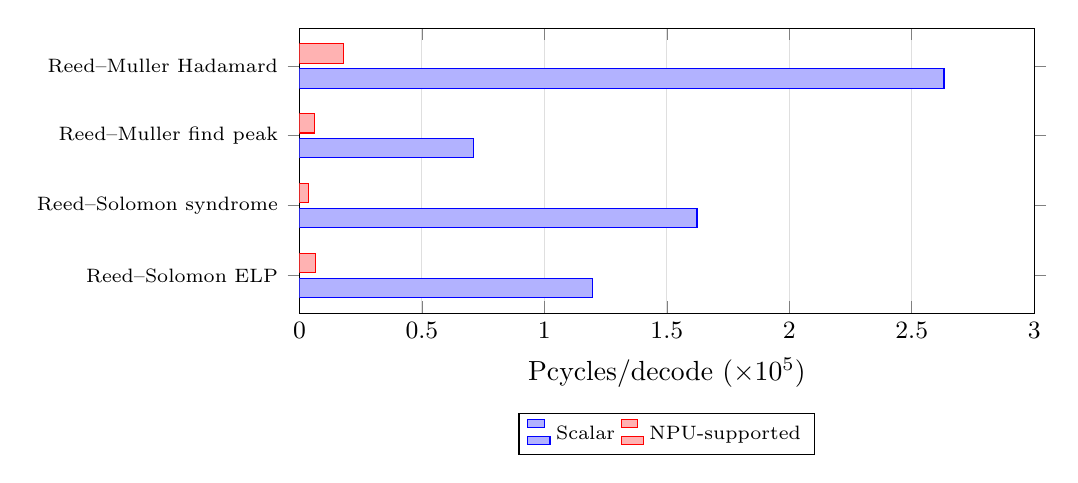
\begin{tikzpicture}
\begin{axis}[
    xbar,
    width=0.9\linewidth,
    height=5.2cm,
    bar width=7pt,
    xlabel={Pcycles/decode $(\times 10^5)$},
    xmin=0,
    xmax=3.0,
    xtick={0,0.5,1.0,1.5,2.0,2.5,3.0},
    scaled x ticks=false,
    symbolic y coords={
        Reed--Muller Hadamard,
        Reed--Muller find peak,
        Reed--Solomon syndrome,
        Reed--Solomon ELP
    },
    ytick=data,
    y dir=reverse,
    enlarge y limits=0.18,
    legend style={
        at={(0.5,-0.35)},
        anchor=north,
        legend columns=2,
        font=\scriptsize
    },
    x tick label style={font=\small},
    yticklabel style={font=\scriptsize},
    xmajorgrids=true,
    grid style={gray!25},
]
\addplot coordinates {
    (2.63175,Reed--Muller Hadamard)
    (0.71217,Reed--Muller find peak)
    (1.62312,Reed--Solomon syndrome)
    (1.19595,Reed--Solomon ELP)
};
\addplot coordinates {
    (0.17950,Reed--Muller Hadamard)
    (0.06081,Reed--Muller find peak)
    (0.03517,Reed--Solomon syndrome)
    (0.06576,Reed--Solomon ELP)
};
\legend{Scalar,NPU-supported}
\end{axis}
\end{tikzpicture}
\vspace{0.5em}
\caption{Comparison of selected optimized decoding substages between the scalar baseline and the NPU-supported backend (ELP is abbreviated for error locator polynomial). Lower is better.}
\label{fig:substage-pcycle-comparison}
\end{figure}



\subsection{Real-Device Results}

The real-device experiments were conducted on a Snapdragon\textregistered{} 8 Gen 2 Mobile Hardware Development Kit, model HDK8550, based on the Qualcomm
Snapdragon SM8550P application processor. According to the manufacturer specification, this platform includes an 8-core 64-bit Kryo CPU, consisting of
one Arm Cortex-X3 prime core up to 3.2 GHz, four performance cores up to 2.8 GHz, and three efficiency cores up to 2.0 GHz. It also includes a Qualcomm
Hexagon processor equipped with Hexagon Vector eXtensions (HVX), scalar and tensor accelerators, micro tile inferencing, Hexagon Direct Link, and support
for INT4, INT8, INT16, and FP16 arithmetic.

The real-device measurements use the corresponding 256-fixture decoding corpus for each HQC parameter set. Unlike the simulator benchmark, which reports
Hexagon Pcycles, the real-device benchmark reports host-observed latency and direct device energy. Each reported value is the mean of five runs, and
each run performs \(32{,}000\) decodes. The NPU-supported backend uses the current non-worker FastRPC path, where one batched remote call executes the
full decode loop on the cDSP. Energy is measured from Android power-supply voltage/current samples with qprof disabled. Here, qprof refers to Qualcomm's profiler for DSP/NPU
utilization and clock-state diagnostics; its measurements are used only as diagnostic evidence and are not used for the energy claims.

\begin{table}[htbp]
\centering
\renewcommand{\arraystretch}{1.15}
\small

\begin{tabular}{|c|c|c|c|c|c|c|}
\hline
\textbf{HQC} & \textbf{Backend} & \textbf{us/decode} & \textbf{uJ/decode} &
\textbf{decodes/s/W} & \textbf{Speedup} & \textbf{Energy gain} \\
\hline
HQC-128 & CPU scalar    & 80.857  & 193.861 & 5,571.312  & 1.00x & 1.0x  \\
\hline
HQC-128 & NPU-supported & 36.254  & 11.260  & 112,102.113 & 2.23x & 17.6x \\
\hline
HQC-192 & CPU scalar    & 103.879 & 244.170 & 4,280.092  & 1.00x & 1.0x  \\
\hline
HQC-192 & NPU-supported & 31.150  & 11.343  & 115,195.952 & 3.33x & 23.1x \\
\hline
HQC-256 & CPU scalar    & 228.148 & 577.240 & 1,772.878  & 1.00x & 1.0x  \\
\hline
HQC-256 & NPU-supported & 56.894  & 23.557  & 56,765.408 & 4.01x & 29.6x \\
\hline
\end{tabular}
\vspace{0.5em}
\caption{Real-device latency, energy, and throughput-per-watt measurements across HQC parameter sets. Values are means over five runs; run-to-run variability is summarized separately in Table~\ref{tab:real-device-stability}.}
\label{tab:real-device-latency-energy}
\end{table}

The decodes/s/W column is computed as \(1/J_{\mathrm{decode}}\) from the direct energy measurement in \(\mu\mathrm{J}/\mathrm{decode}\). Across all three HQC parameter sets, the NPU-supported backend improves both latency and energy efficiency over the scalar CPU baseline. The measured speedup is \(2.23\times\) to \(4.01\times\), and the energy gain is \(17.6\times\) to \(29.6\times\). The HQC-192 NPU-supported row is faster than HQC-128 on the real device even though the simulator reports a larger compute cost; this inversion is likely caused by system-level effects such as FastRPC batching, cDSP clock behavior, cache state, and direct-power sampling rather than by a lower intrinsic HQC-192 compute cost.

\begin{table}[htbp]
\centering
\renewcommand{\arraystretch}{1.15}
\small
\begin{tabular}{|c|c|c|c|c|}
\hline
\textbf{HQC} & \textbf{Backend} & \textbf{us/decode CV} &
\textbf{uJ/decode CV} & \textbf{CPU ms/decode CV} \\
\hline
HQC-128 & CPU scalar    & 0.26\% & 4.23\% & 0.75\% \\
\hline
HQC-128 & NPU-supported & 0.03\% & 16.70\% & 37.27\% \\
\hline
HQC-192 & CPU scalar    & 0.31\% & 4.17\% & 0.85\% \\
\hline
HQC-192 & NPU-supported & 0.40\% & 30.76\% & 71.26\% \\
\hline
HQC-256 & CPU scalar    & 0.08\% & 2.95\% & 0.49\% \\
\hline
HQC-256 & NPU-supported & 0.31\% & 54.32\% & 22.82\% \\
\hline
\end{tabular}
\vspace{0.5em}
\caption{Run-to-run variability for the direct real-device measurements, reported as coefficient of variation \(\mathrm{CV}=\sigma/\mu\). Latency is stable across runs; energy has higher variability because it is derived from board-level power samples.}
\label{tab:real-device-stability}
\end{table}

\begin{figure}[h]
\centering
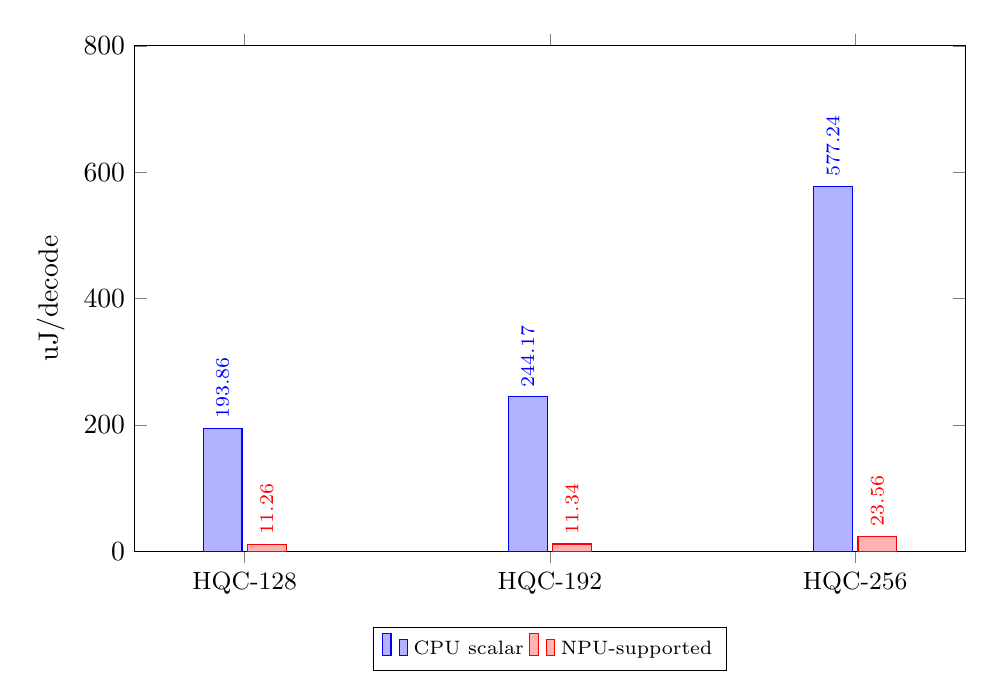
\begin{tikzpicture}
\begin{axis}[
    ybar,
    width=\linewidth,
    height=8cm,
    bar width=14pt,
    ylabel={uJ/decode},
    symbolic x coords={HQC-128,HQC-192,HQC-256},
    xtick=data,
    ymin=0,
    ymax=800,
    enlarge x limits=0.18,
    legend style={at={(0.5,-0.15)},anchor=north,legend columns=2,font=\scriptsize},
    nodes near coords,
    nodes near coords style={font=\scriptsize,rotate=90,anchor=west},
    yticklabel style={/pgf/number format/fixed},
    x tick label style={font=\small},
]
\addplot coordinates {
    (HQC-128,193.861)
    (HQC-192,244.170)
    (HQC-256,577.240)
};

\addplot coordinates {
    (HQC-128,11.260)
    (HQC-192,11.343)
    (HQC-256,23.557)
};

\legend{CPU scalar,NPU-supported}
\end{axis}
\end{tikzpicture}
\caption{Real-device energy per decode. Lower is better.}
\label{fig:real-device-energy}
\end{figure}

In addition to latency and energy, Table~\ref{tab:real-device-cpu-offload}
reports the CPU time consumed by the benchmark host process itself. These
numbers are collected by wrapping the benchmark with
\texttt{scripts/measure\_process\_cpu.sh}. The script samples the process and
thread accounting files under \texttt{/proc/<pid>/task/*/stat} while the
benchmark is running, sums user and system CPU ticks, and converts them to
milliseconds using the Linux clock tick rate. The same wrapper is used for both
backends: for CPU scalar, the measured process runs the scalar decoder directly;
for NPU-supported, the measured process mostly submits FastRPC work to the cDSP
and waits for completion.

The \textbf{process CPU \%} column is the sampled host CPU time divided by the
wall-clock runtime of the benchmark. It is normalized to one CPU core: \(100\%\)
means the process kept one CPU core fully busy on average, not the whole
multi-core SoC. The \textbf{CPU ms/decode} column is the same host CPU time
divided by the number of completed decodes. The \textbf{CPU reduction} column is
computed from CPU ms/decode as
\[
100 \times
\left(
1 -
\frac{\mathrm{CPU\ ms/decode}_{\mathrm{NPU}}}
     {\mathrm{CPU\ ms/decode}_{\mathrm{scalar}}}
\right).
\]
It therefore measures host-side CPU offload only; the NPU-supported decoder
still consumes Hexagon cycles on the cDSP.

\begin{table}[htbp]
\centering
\renewcommand{\arraystretch}{1.15}
\small
\begin{tabular}{|c|c|c|c|c|}
\hline
\textbf{HQC} & \textbf{Backend} & \textbf{process CPU \%} &
\textbf{CPU ms/decode} & \textbf{CPU reduction} \\
\hline
HQC-128 & CPU scalar    & 93.884 & 0.0796250 & 0.000\% \\
\hline
HQC-128 & NPU-supported & 1.714  & 0.0007500 & 99.059\% \\
\hline
HQC-192 & CPU scalar    & 94.477 & 0.1025625 & 0.000\% \\
\hline
HQC-192 & NPU-supported & 1.275  & 0.0005000 & 99.512\% \\
\hline
HQC-256 & CPU scalar    & 97.484 & 0.2274375 & 0.000\% \\
\hline
HQC-256 & NPU-supported & 1.195  & 0.0007500 & 99.670\% \\
\hline
\end{tabular}
\vspace{0.5em}
\caption{Process-level CPU utilization and CPU-time reduction on the real device.}
\label{tab:real-device-cpu-offload}

\end{table}

The process-level CPU measurements show why CPU offloading matters beyond energy
alone. When the CPU consumes nearly all of one core decoding HQC, the host has
less room for other application or system work. Moving the decoding workload to
the NPU reduces host CPU ms/decode by \(99.1\%\)--\(99.7\%\) across all HQC
parameter sets. This reduction is a host-side offload metric only; the
NPU-supported decode still consumes Hexagon cycles, which are reflected in the
latency and energy measurements above.

We also isolate the FastRPC boundary cost. The batched row uses the same
non-worker batched decode benchmark as the real-device latency table, while the
``decode-one'' experiment makes one FastRPC call per decode. Table
\ref{tab:fastrpc-boundary-overhead} reports only the boundary-sensitive modes:
a no-op ping, one-decode-per-RPC, and the batched path used to
quantify boundary amortization.

\begin{table}[htbp]
\centering
\renewcommand{\arraystretch}{1.15}
\small

\begin{tabular}{|c|c|c|c|c|}
\hline
\textbf{HQC} & \textbf{Ping us/RPC} & \textbf{Decode-one us/decode} &
\textbf{Batched us/decode} & \textbf{Decode-one slowdown} \\
\hline
HQC-128 & 556.926 & 603.010 & 36.260 & 16.63x \\
\hline
HQC-192 & 556.958 & 598.996 & 31.659 & 18.92x \\
\hline
HQC-256 & 557.411 & 604.529 & 57.584 & 10.50x \\
\hline
\end{tabular}
\vspace{0.5em}
\caption{FastRPC boundary overhead on the real device. Values are means over five runs; variability is summarized separately in Table~\ref{tab:fastrpc-boundary-stability}.}
\label{tab:fastrpc-boundary-overhead}
\end{table}

\begin{table}[htbp]
\centering
\renewcommand{\arraystretch}{1.15}
\small
\begin{tabular}{|c|c|c|c|}
\hline
\textbf{HQC} & \textbf{Ping CV} & \textbf{Decode-one CV} &
\textbf{Batched CV} \\
\hline
HQC-128 & 0.55\% & 3.26\% & 0.04\% \\
\hline
HQC-192 & 0.87\% & 2.50\% & 0.42\% \\
\hline
HQC-256 & 1.52\% & 1.12\% & 0.27\% \\
\hline
\end{tabular}
\vspace{0.5em}
\caption{Run-to-run variability for the FastRPC boundary measurements, reported as coefficient of variation \(\mathrm{CV}=\sigma/\mu\).}
\label{tab:fastrpc-boundary-stability}
\end{table}

The FastRPC no-op boundary alone is about \(557\ \mu\mathrm{s}\) per call, which
is much larger than the batched per-decode cost for all three HQC parameter
sets. Calling FastRPC once per decapsulation is therefore \(10.50\times\) to
\(18.92\times\) slower than batching the decode loop inside one remote call.
Representative cached payload movement remains secondary to the boundary
itself: the measured cached input overhead is on the order of \(580\)--\(610\ \mu\mathrm{s}\)
per RPC for the current build. Thus, the real-device NPU numbers
should be interpreted as batched cDSP throughput with heavily amortized FastRPC
overhead, not as the latency of an API that performs one remote call per
decapsulation.
    
